In this section we summarize the magnetic field simulations for use of the BaBar solenoid in ECCE.  These simulations were performed by Paul Brindza of Thomas Jefferson National Laboratory using the Opera computational tool. 

\subsection{ECCE Flux Return Configuration}

Simulations of the ECCE magnetic field configuration were done using OPERA (Tosca) for a central magnetic field of 1.5T, corresponding to a stored energy of $2.44\times 10^{7} J$.  Figure~\ref{fig:3DModel} shows the geometry of the 3D model for the OPERA calculations, while Figure~\ref{fig:BzOnAxis} shows the z component of the magnetic field along the central axis of the solenoid. 

\begin{figure}[h!tbp]
    \centering
    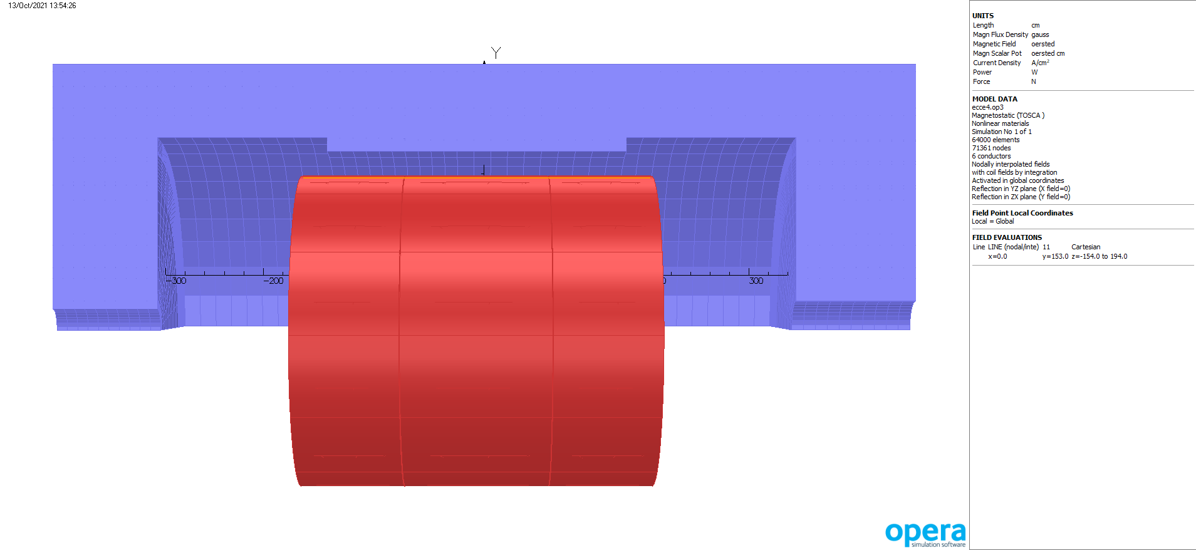
\includegraphics[width=0.9\textwidth]{figs/3DModel.png}
    \caption{Image of the 3D model used for magnetic field calculations within OPERA. Shown are the coil (red) and a cutaway of the flux return (blue). Note the asymmetric nature of the flux return on the forward going (right) side of the coil. }
    \label{fig:3DModel}
\end{figure}

\begin{figure}[h!tbp]
    \centering
    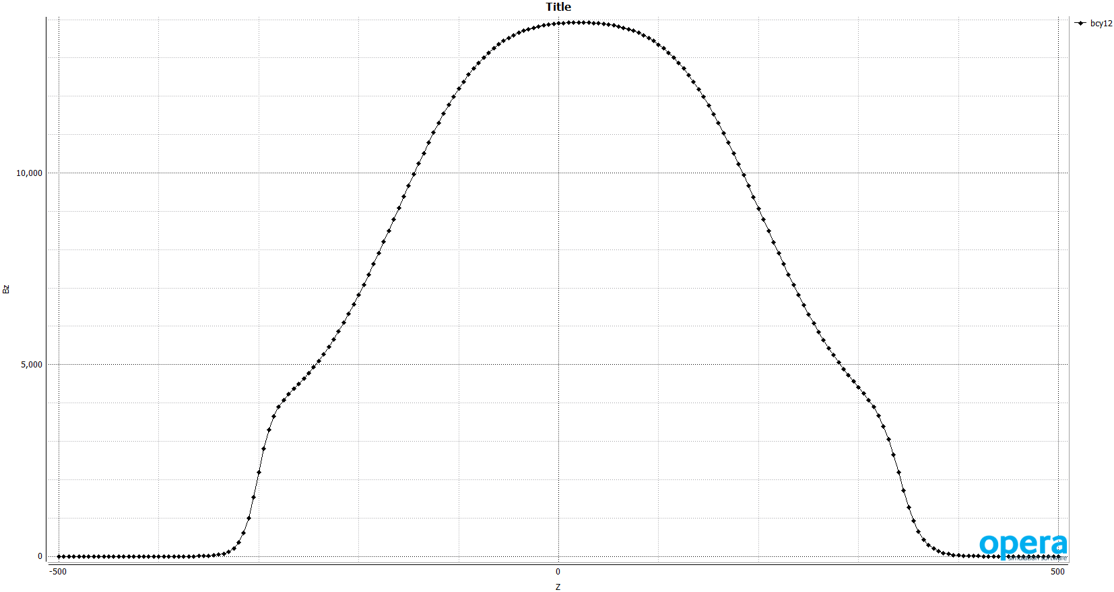
\includegraphics[width=0.9\textwidth]{figs/BzOnAxis.png}
    \caption{Magnetic field along the z-axis in the ECCE magnet.  Note that the coil is shifted in z with respect to the center of the coordinate system by +20cm. }
    \label{fig:BzOnAxis}
\end{figure}

\subsection{Estimated Forces on the BaBar Coils}

The asymmetric nature of the ECCE detector flux return will yield an asymmetric force on the BaBar solenoid coils. Forces on the magnet coils due to the asymetric arrangement were calculated within OPERA using the integral method (most accurate) and checked using hand calculations. Figure~\ref{fig:BRadial} shows the radial component of the magnetic field at the location of the solenoid coils. This component of the magnetic field will generate longitudinal stress on the coils. Figure~\ref{fig:BzThroughCoil} shows the z-component of the magnetic field at the location of the solenoid coils. This component of the magnetic field will generate a radial "hoop" stress on the coils. 

\begin{figure}[h!tbp]
    \centering
    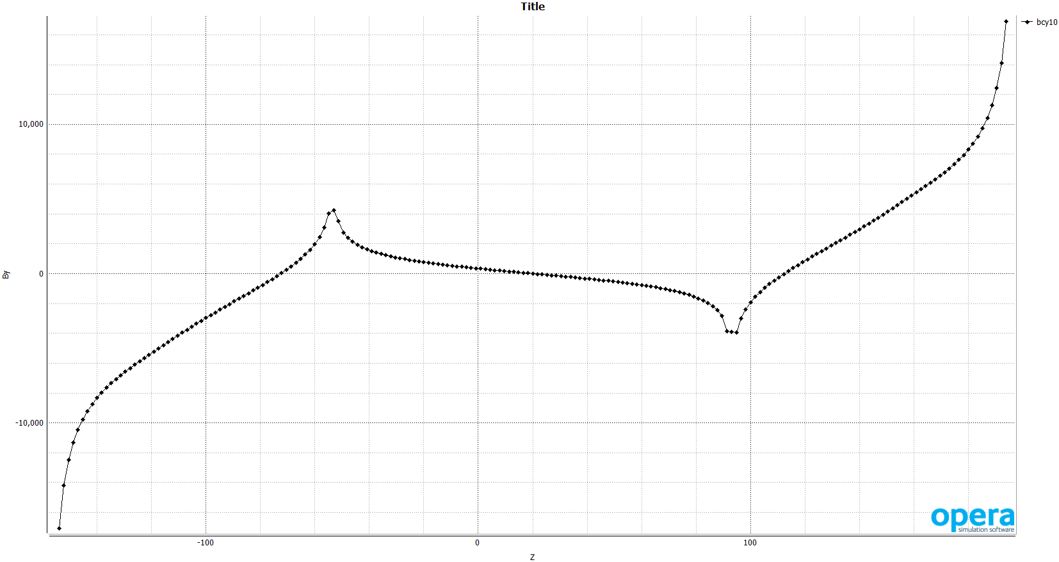
\includegraphics[width=0.9\textwidth]{figs/BRadial.png}
    \caption{Radial component of the magnetic field at the coil location of $r=153cm$ along a line parallel to the z-axis from $z=-154cm$ to $z=194cm$.  }
    \label{fig:BRadial}
\end{figure}

\begin{figure}[h!tbp]
    \centering
    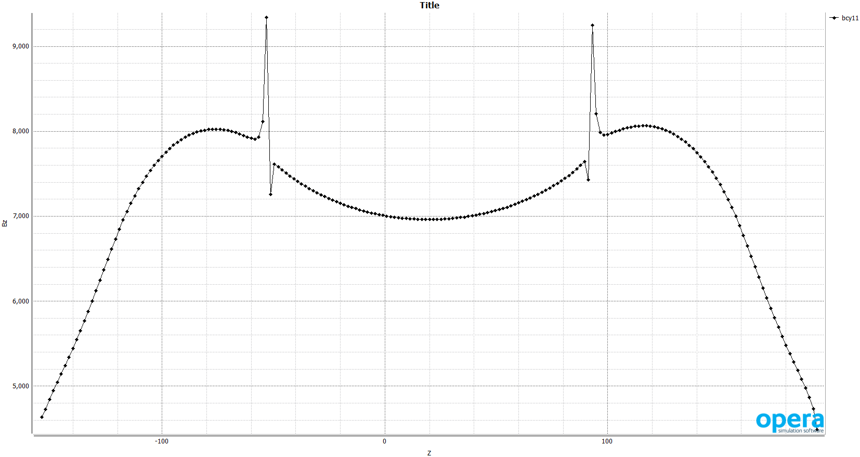
\includegraphics[width=0.9\textwidth]{figs/BzThroughCoil.png}
    \caption{Component of the magnetic field along the z-axis at the coil location of $r=153cm$ along a line parallel to the z-axis from $z=-154cm$ to $z=194cm$.  }
    \label{fig:BzThroughCoil}
\end{figure}

Table~\ref{tab:opera_forces} shows the force on each coil and the net force on the magnet calculated from OPERA using the integral method.  The unbalanced force on the magnet is 3600N (or 810lbs).  As a comparison, a hand calculation of the net forces on the coils is shown in Table~\ref{tab:hand_forces}, which yields a net force of 4211N (or 947 lbs).  It should be noted that the field differences that generate these forces are less than the model accuracy of 1.5\%. Overall, the unbalanced forces on the magnet are small because the magnetic field at the locations of the forward/backward calorimeters are small and most of the magnetic flux is returned through the barrel.  These small forces should not present a substantial engineering difficulty in the proposed ECCE configuration. 

\begin{table}
\centering
\begin{tabular}{c|c|c}
Coil & Location & Force (NT) \\
\hline
1 & center inner & 5988 \\
2 & center outer & 817 \\
3 & left(-) inner & 3,073,723 \\
4 & right(+) inner & -3,072,571 \\
5 & left(-) outer & 3,085,758 \\
6 & right(+) outer & 3,082,957 \\
\hline
Net Force & center inner & -3600 \\
Net Force (lbs) & center inner & 810 lbs \\
\end{tabular}
\caption{Coil forces calculated from field integrals in OPERA.}
\label{tab:opera_forces}
\end{table}

\begin{table}
\centering
\begin{tabular}{c|c|c|c}
Coils & Net $B_{avg}$ T & I (amps) & Force (NT) \\
\hline
1\&2 (center) & -0.00035 & -1484508 & +5022 \\
3\&5 (neg. side) & -0.39507 & -1709732 & +6,493,359 \\
1\&2 (pos. side) & +0.39563 & -1709711 & -6,502,592 \\
\hline
Total & $+1.47\times10^{-5}$ & -4903951 & -4211 \\
\end{tabular}
\caption{Net forces on coil pairs from a hand calculation using the average magnetic field using $F=B_{r}IL$, where $L=9.61m$.}
\label{tab:hand_forces}
\end{table}
